\documentclass[a4paper, 12pt]{article}
\usepackage[a4paper,top=1.0cm, bottom=0.5cm, left=0.25cm, right=0.75cm]{geometry}
\usepackage[utf8]{inputenc}
\usepackage{mathtext}
\usepackage{amsmath}
\usepackage{amsfonts}
\usepackage[english, russian]{babel}
\usepackage{indentfirst}
\usepackage{longtable}
\usepackage{graphicx}
\graphicspath{{pictures/}}
\DeclareGraphicsExtensions{.pdf,.png,.jpg}
\usepackage{natbib}
\usepackage{mathrsfs}
\usepackage[europeanresistors, americaninductors]{circuitikz}

\title{Лабораторная работа 2.5.1 Измерение коэффициента поверхностного натяжения жидкости.}
\author{Михаил Колтаков}
\date{16 февраля 2020 г.}

\begin{document}
	\maketitle
	\section*{Цель работы}
		1) измерение температурной зависимости  коэффициента поверхностного натяжения дистиллированной воды с использованием известного коэффициента поверхностного натяжения спирта;  2) определение полной поверхностной энергии  и теплоты, необходимой для изотермического образования единицы  поверхности жидкости  при различной температуре.
	\section*{Оборудование}
		Прибор Ребиндера с термостатом и микроманометром, спирт и вода, стакан.
	\section*{Теория к работе}
		Наличие поверхностного слоя приводит к различию давлений по разные стороны от искривленной границы раздела двух сред.  Для сферического пузырька с воздухом  внутри жидкости избыточное давление даётся формулой Лапласа: 
		$$\Delta P = P_{внутри} - P_{снаружи} = \frac{2 \sigma}{R}$$
		$\sigma$ - коэффициент поверхностного натяжения, $R$ - радиус кривизны поверхности раздела двух фаз. Измеряется давление $\Delta P$, необходимое для выталкивания в жидкость пузырька воздуха. 
	\section*{Описание экспериментальной установки}
		На рисунке ниже изображена экспериментальная установка. Исследуемая жидкость(дистиллиро- ванная вода) наливается в сосуд(колбу) В. Тестовая жидкость(этиловый спирт) наливается в сосуд Е. При измерениях колбы герметично закрываются пробками. Через одну из двух пробок проходит полая металлическая игла С. Этой пробкой закрывается сосуд, в котором проводятся измерения. Верхний конец иглы открыт в атмосферу, а нижний погружён в жидкость. Другой сосуд герметично закрывается второй пробкой. При создании достаточного разряжения воздуха в колбе с иглой пузырьки воздуха начинают пробулькивать через жидкость. Поверхностное натяжение можно определить по величине разряжения $\Delta P$, необходимого для прохождения пузырьков(при известном радиусе иглы).
		\\
		\\
		Разряжение в системе создается с помощью аспиратора А. Кран К2 разделяет две полости аспиратора. При закрытом кране К2 открывают кран К1, разряжение воздуха в колбе создаётся когда вода вытекает из крана К1 по каплям. В колбах В и С, соединённых трубками с нижней полостью аспиратора, создается такое же пониженное давление. Разность давлений в полостях с разряженным воздухом и атмосферой измеряется спиртовым микроманометром. Для стабилизации температуры исследуемой жидкости через рубашку D колбы В непрерывно прогоняется вода из термостата. 
		\begin{figure}[h]
			\center{\includegraphics{exp}}
		\end{figure}
		\\
		\\
		Обычно кончик иглы лишь касается поверхности жидкости, чтобы исключить влияние гидростатического давления столба жидкости. Однако при измерении температурной зависимости коэффициента поверхностного натяжения возникает ряд сложностей. Во-первых, большая теплопроводность металлической трубки приводит к тому, что температура на конце трубки заметно ниже, чем в глубине жидкости. Во-вторых, тепловое расширение поднимает уровень жидкости при увеличении температуры.
		\\
		\\
		Обе погрешности можно устранить, погрузив кончик трубки глубже в жидкость. Полное давление, измеренное при этом микроманометром, $P = \Delta P + \rho gh$. $\rho gh$ не зависит от температуры жидкости. Величину $\rho gh$ следует измерить двумя способами. Во-первых, замерить величину $Р1= \Delta P'$, когда кончик трубки только касается поверхности жидкости. Затем при этой же температуре опустить иглу глубже в жидкость и замерить $Р2 = \rho gh + \Delta P"$ ($\Delta P'$, $\Delta P"$ – давление Лапласа). Из-за несжимаемости жидкости можно положить $\Delta P'= \Delta P"$ и тогда $\rho gh = Р2 - Р1$. Во-вторых, при измерениях Р1 и Р2 замерить линейкой глубину погружения иглы h.
		
	\section*{Ход работы}
		Измерим $d = 2R = 1,10 \pm 0,05$мм - диаметр иглы.
		Разность давлений измеряется не напрямую, а через положение жидкости в манометре, поэтому $\Delta P = k h$, где h - высота в миллиметрах жидкости в манометре, а $k = 1587,697 \frac{кг}{м^2 \cdot с^2}$ - коэффициент пересчёта. Измеренные данные занесём в таблицу:
		\begin{longtable}[H]{|c|c|c|c||c|c|c|c|}
			\hline
			Жидкость & h, мм & $\Delta P$, Па & $\overline{\Delta P}$ - $\rho gh$, Па & Жидкость & h, мм & $\Delta P$, Па & $\overline{\Delta P}$ - $\rho gh$, Па \\
			\hline
			& 44 & 69,86 & &  & 89 & 141,31 & \\
			& 43 & 68,27 & &  & 88 & 139,72 & \\
			Спирт(22 °C) & 43 & 68,27 & 68,91 & Поверхность воды(22 °C) & 87 & 138,13 & 138,13 \\
			& 44 & 69,86 & (без &  & 86 & 136,54 & (без  \\
			& 43 & 68,27 & вычитания) &  & 85 & 134,95 & вычитания) \\
			\hline
			& 124 & 196,87 & &  & 123 & 195,28 & \\
			& 124 & 196,87 & &  & 124 & 196,87 & \\
			Вода(22 °C) & 124 & 196,87 & 138,13 & Вода(26 °C) & 124 & 196,87 & 142,34\\
			& 124 & 196,87 & &  & 123 & 195,28 & \\
			& 124 & 196,87 & &  & 124 & 196,87 & \\
			\hline
			& 123 & 195,28 & &  & 122 & 193,69 & \\
			& 124 & 196,87 & &  & 122 & 193,69 & \\
			Вода(30 °C) & 123 & 195,28 & 141,70 & Вода(34 °C) & 122 & 193,69 & 139,80\\
			& 123 & 195,28 & &  & 122 & 193,69 & \\
			& 123 & 195,28 & &  & 122 & 193,69 & \\
			\hline
			& 121 & 192,11 & &  & 120 & 190,52 & \\
			& 121 & 192,11 & &  & 120 & 190,52 & \\
			Вода(38 °C) & 121 & 192,11 & 138,21 & Вода(42 °C) & 120 & 190,52 & 136,62 \\
			& 121 & 192,11 & &  & 120 & 190,52 & \\
			& 121 & 192,11 & &  & 120 & 190,52 & \\
			\hline
			& 119 & 188,94 & &  &  &  & \\
			& 119 & 188,94 & &  &  &  & \\
			Вода(46 °C) & 119 & 188,94 & 135,04 &  &  &  & \\
			& 119 & 188,94 & &  &  &  & \\
			& 119 & 188,94 & &  &  &  & \\
			\hline 
		\end{longtable}
		Из таблицы находим $\rho gh = 52,74\: Па$. Также из данного коэффициента поверхностного натяжения для этилового спирта находим, что диаметр трубки равен $d_{сп}=1,27$ мм. Погрешность составила 15$\%$. Из разности высот иглы рассчитаем $\rho gh_2 = 49.05$ Теперь построим таблицу зависимости $\sigma (T)$. Погрешность нахождения $\sigma$ равна $\Delta \sigma = 0,33$ мН/м. 
		\begin{longtable}[H]{|c|c|c|c|c|c|c|c|}
			\hline
			T, °C & 22 & 26 & 30 & 34 & 38 & 42 & 46 \\
			\hline
			$\sigma$, мН/м & 78,63 & 78,29 & 77,94 & 76,89 & 76,02 & 75,14 & 74,27 \\
			\hline
		\end{longtable}
	
		Построим график зависимости $\sigma (T)$:
		
		\begin{figure}[h]
			\center{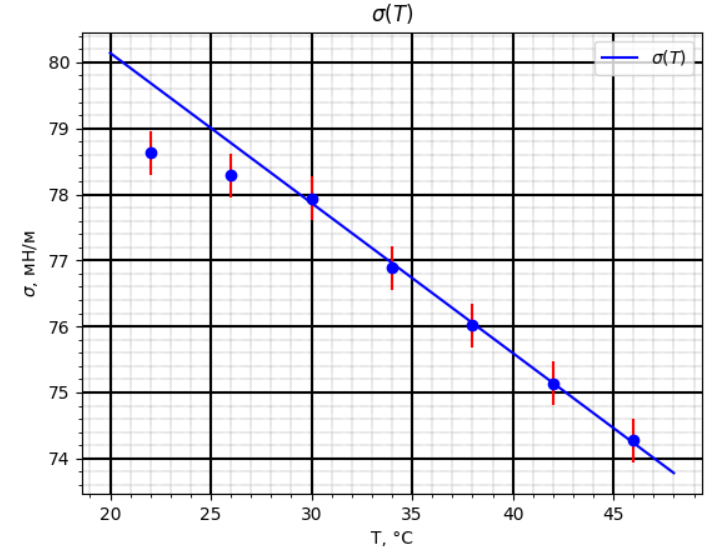
\includegraphics{S(T)}}
		\end{figure}
	
		По этому графику можно найти $\frac{d \sigma}{dT} = -0,23 \pm 0,3\: \frac{мН}{м \cdot K}$. Теоретически рассчитанное значение составляет -0,21 $\frac{мН}{м \cdot K}$. Теперь на другом графике построим q(T) и $\frac{U}{F} (T)$:
		\begin{figure}[h]
			\center{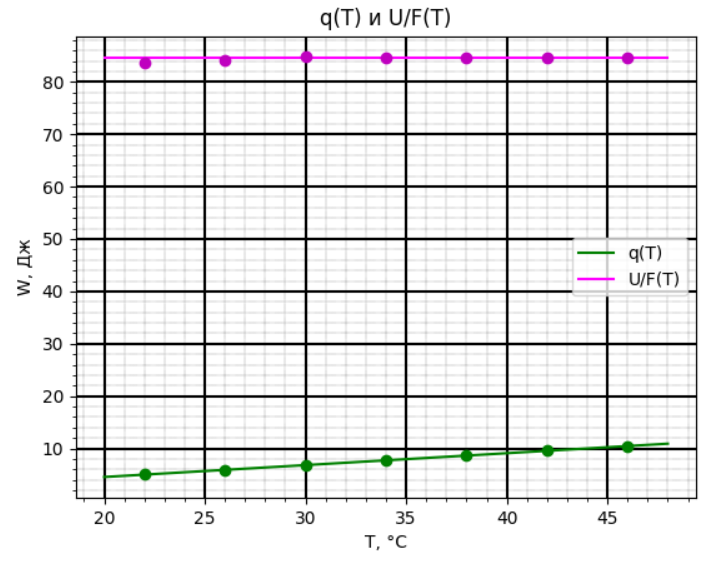
\includegraphics{q(T)}}
		\end{figure}
	\section*{Вывод}
		Нам удалось измерить зависимость коэффициента поверхностного натяжения от температуры. Значение $\frac{d \sigma}{dT}$ сошлось с табличным, однако значение самого коэффициента поверхностного натяжения $\sigma$ оказалось несколько выше табличного. Предположив линейность зависимости $\sigma (T)$, мы получили, что критическая температура исследуемой жидкости равна 373 °C, когда у дистиллированной воды она равна 374 °C. Неточности в самом значении коэффициента можно объяснить несовершенной чистотой дистиллята. Также удалось определить зависимости полной поверхностной энергии и теплоты, необходимой для изотермического образования единицы поверхности жидкости от температуры и построить их графики. 
\end{document}
